\documentclass[12pt] {article}
\usepackage{times}
\usepackage[margin=1in,bottom=1in,top=0.6in]{geometry}

\usepackage{hhline}
\usepackage{subfig}
\usepackage{amsmath}
\usepackage{amsfonts}
\usepackage[inline,shortlabels]{enumitem}%enumerate with letters
\usepackage{mathrsfs} 
\usepackage[square,numbers]{natbib}
\usepackage{graphicx}
\bibliographystyle{unsrtnat}

\usepackage[framed,numbered,autolinebreaks,useliterate]{./mcode}

\begin{document}

\title{EEC 289Q – Data Analytics for Computer Engineers \\ Homework 1}
\author{Ahmed Mahmoud}
\date{April, 20th 2018} 

\maketitle




%============Table========
%\begin{figure}[tbh]
% \centering    
%\begin{tabular}{ |p{4cm}|| p{2cm}|p{2cm}|p{2cm}|p{2cm}|}
% \hline
% & Processor 1 &  Processor 2  & Processor 3 & Processor 4\\ \hhline{|=|=|=|=|=|}
% \hline
% Performance          &$1.08$        &$1.425$       &\textbf{1.52}  &   \\
% \hline
%\end{tabular} 
%\caption{Metric table for the four processors}
%   \label{tab:metric}
%\end{figure} 
%============Figure========
%\begin{figure}[!tbh]
%\centering        
%   \subfloat {\includegraphics[width=0.65\textwidth]{fig2_4.png}}
%   \caption{ }
%   \label{fig:fig}
%\end{figure}


The following shows the parameter vector 
$$\theta =[35.3222,\ -0.1051,\ 0.0427,\ -0.0205,\ 2.0211,\ -17.8506,\ 4.1607,\ -0.0053,\cdots$$
$$\ -1.4145,\ 0.2570,\ -0.0113,\ -0.9769,\ 0.0073,\ -0.4595]$$

Figure~\ref{fig:fig} shows the graph of the predicated vs. actual prices using linear regression method on houses data of 14 features and 506 data points where 400 are used for training and the rest for testing. The following listing show the modified code for computing the objective function and the gradient. 

\begin{figure}[!tbh]
\centering        
   \subfloat {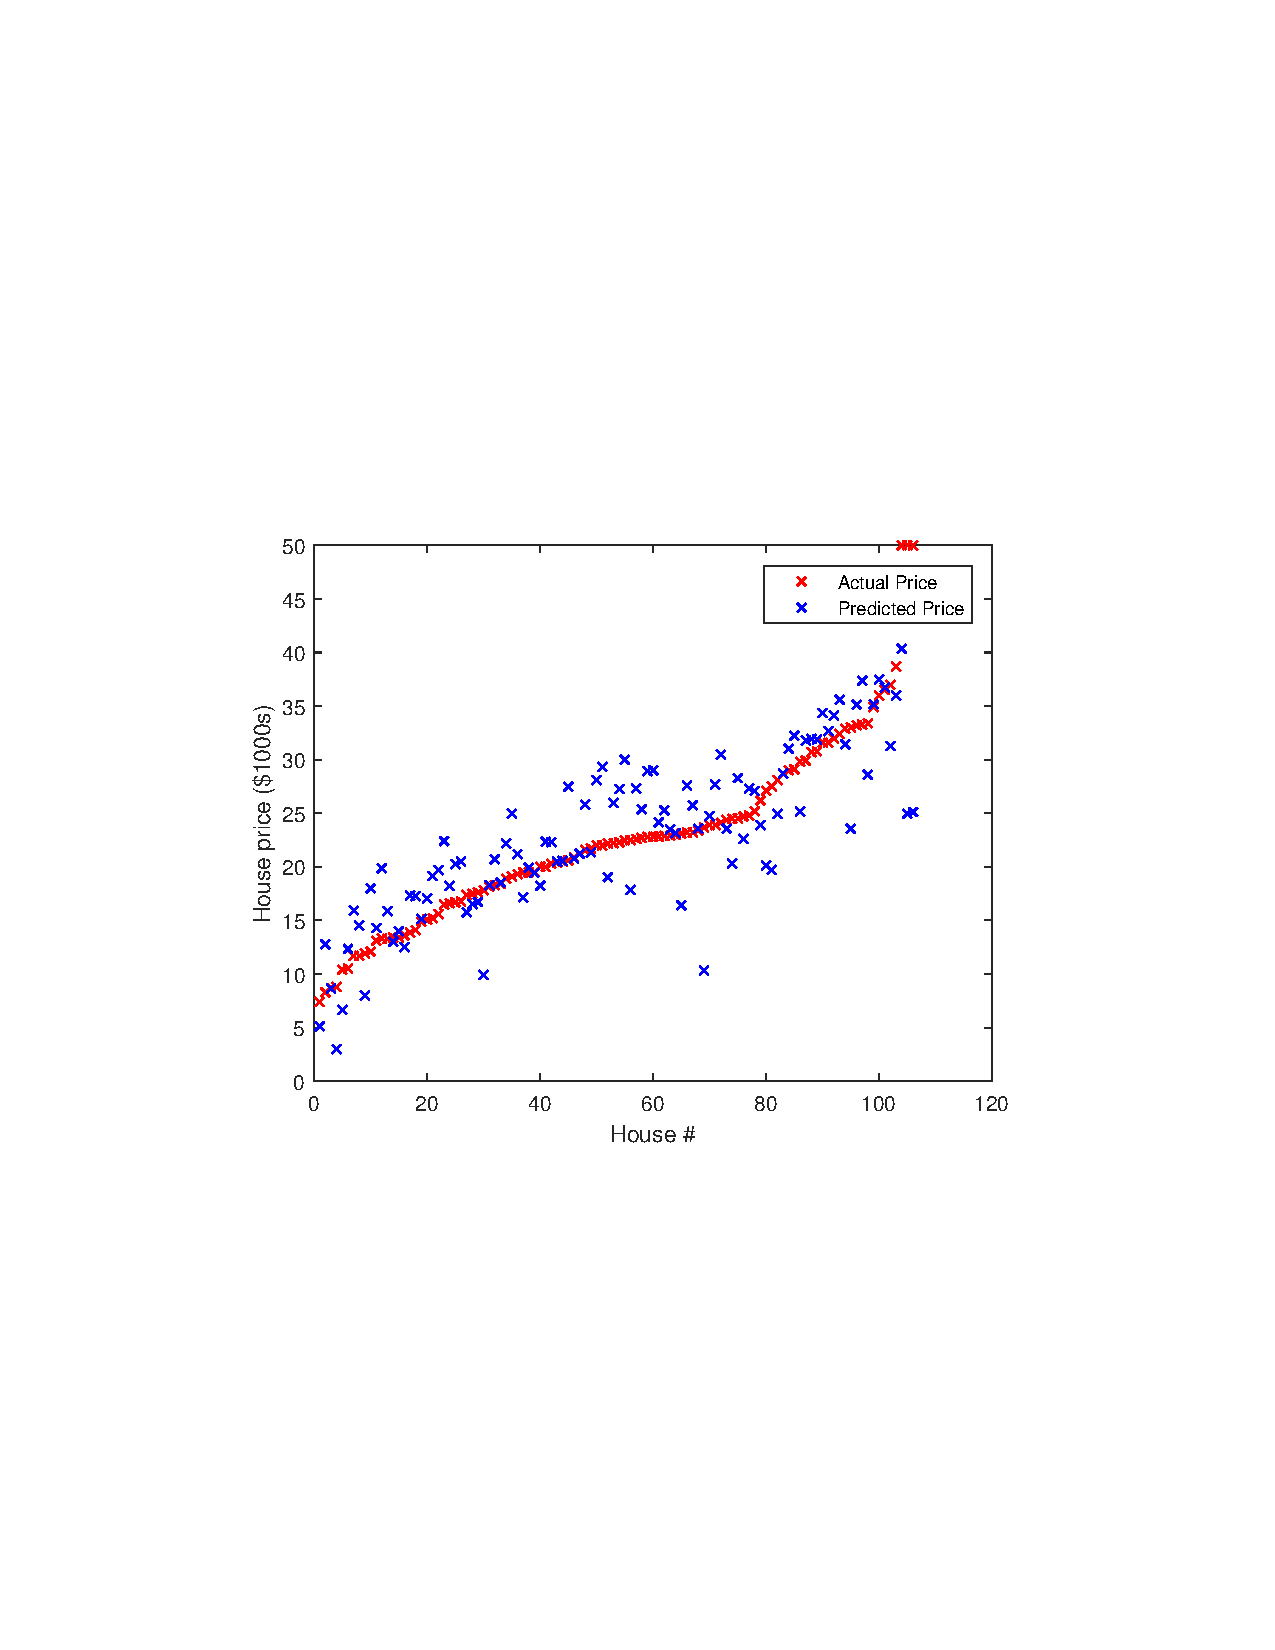
\includegraphics[width=0.75\textwidth]{predict.pdf}}
   \caption{ Predicated vs. actual price using linear regression to predicate the house price.}
   \label{fig:fig}
\end{figure}

\newpage
\begin{lstlisting}
function [f,g] = linear_regression(theta, X,y)
  %
  % Arguments:
  %   theta - A vector containing the parameter values to optimize.
  %   X - The examples stored in a matrix.
  %       X(i,j) is the i'th coordinate of the j'th example.
  %   y - The target value for each example.  y(j) is the target for example j.
  %
  
  m=size(X,2);
  n=size(X,1);

  f=0;
  g=zeros(size(theta));

  %
  % TODO:  Compute the linear regression objective by looping over the examples in X.
  %        Store the objective function value in 'f'.
  %
  % TODO:  Compute the gradient of the objective with respect to theta by looping over
  %        the examples in X and adding up the gradient for each example.  Store the
  %        computed gradient in 'g'.
  
%%% YOUR CODE HERE %%%
    %error vector
    err=theta'*X-y;
    
    %objective function = 0.5*sum((error vector)^2) 
    %using dot product instead
    f=1/2*err*err';
    
    %gradient vector = sum(x*(error vector))
    %using dot product instead
    g=X*err';
end
\end{lstlisting}


\end{document}
